\section{Empirical spectrophotometric models}

\noindent In this section we will be diving into the historical approach of modeling supernova lightcurves. Then we will describe the different models trained 
on photometric and spectroscopic data, which is the usual approach when trying to conduct a cosmological analysis. Finally we will describe the models trained 
on a unique dataset, named the SNfactory dataset. \\


\subsection{Historical approach to modeling lightcurves}

The key information in doing a cosmological analysis with Type Ia supernova is found in their restframe fluxes. The observed fluxes are redshifted meaning that
one must account for their shift in wavelength and duration. We can highlight this in Figure \ref{fig:flux_evolution} where we can see the effects of redshifts on the fluxes.

\begin{figure}[ht]
    \centering
    %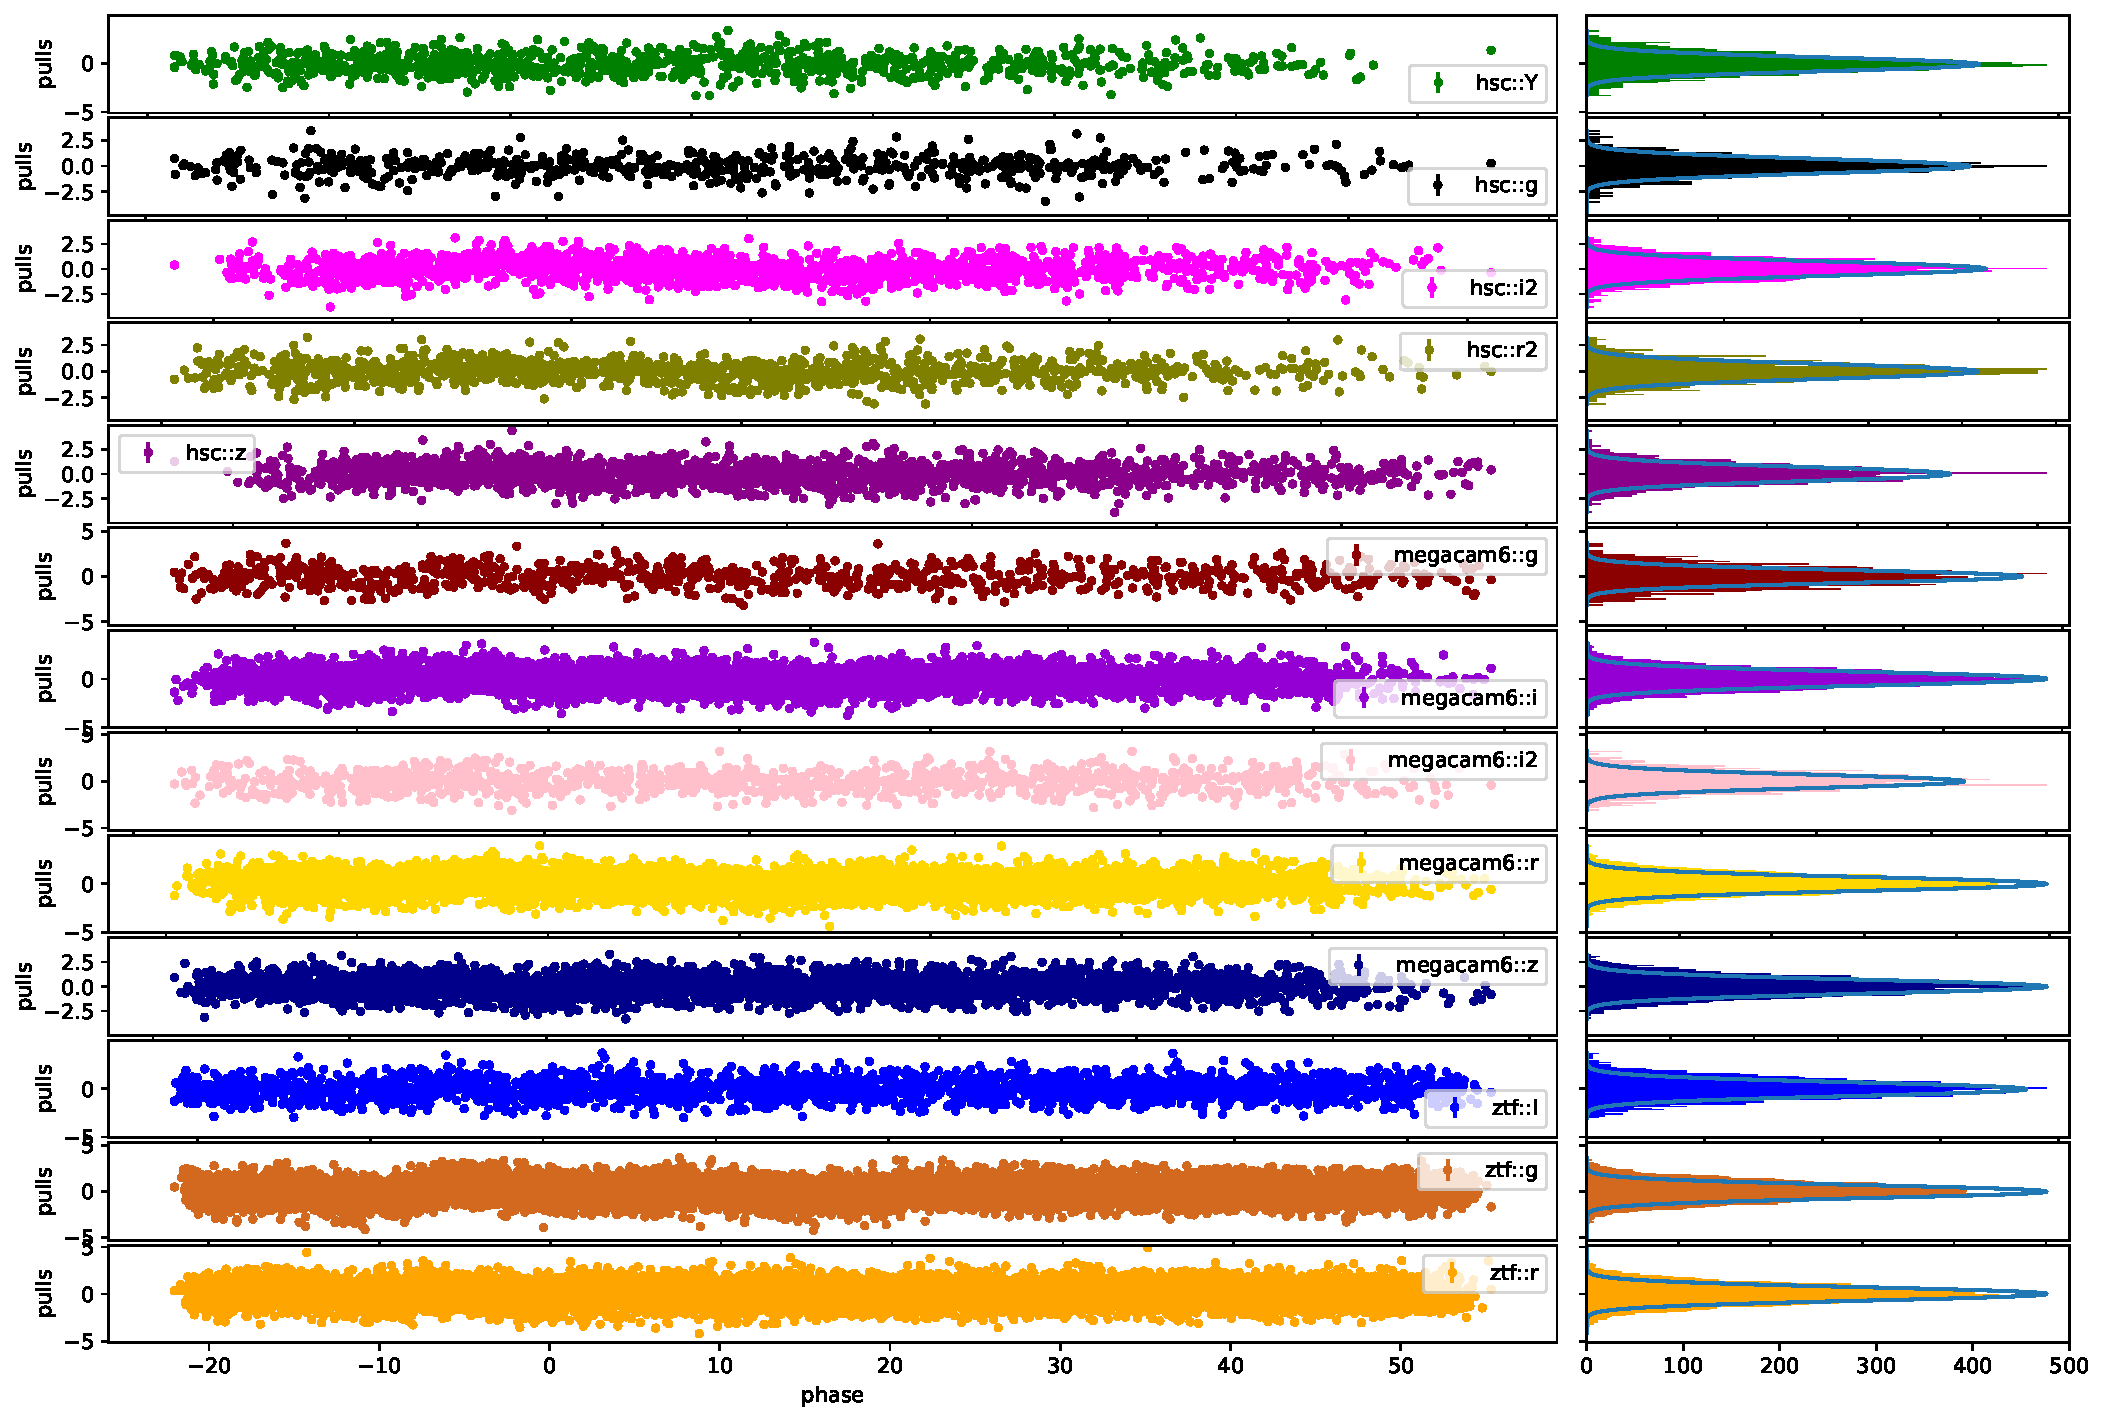
\includegraphics[width=1\textwidth]{MainLayout/DC_chapter/figures/band_resid.pdf}
    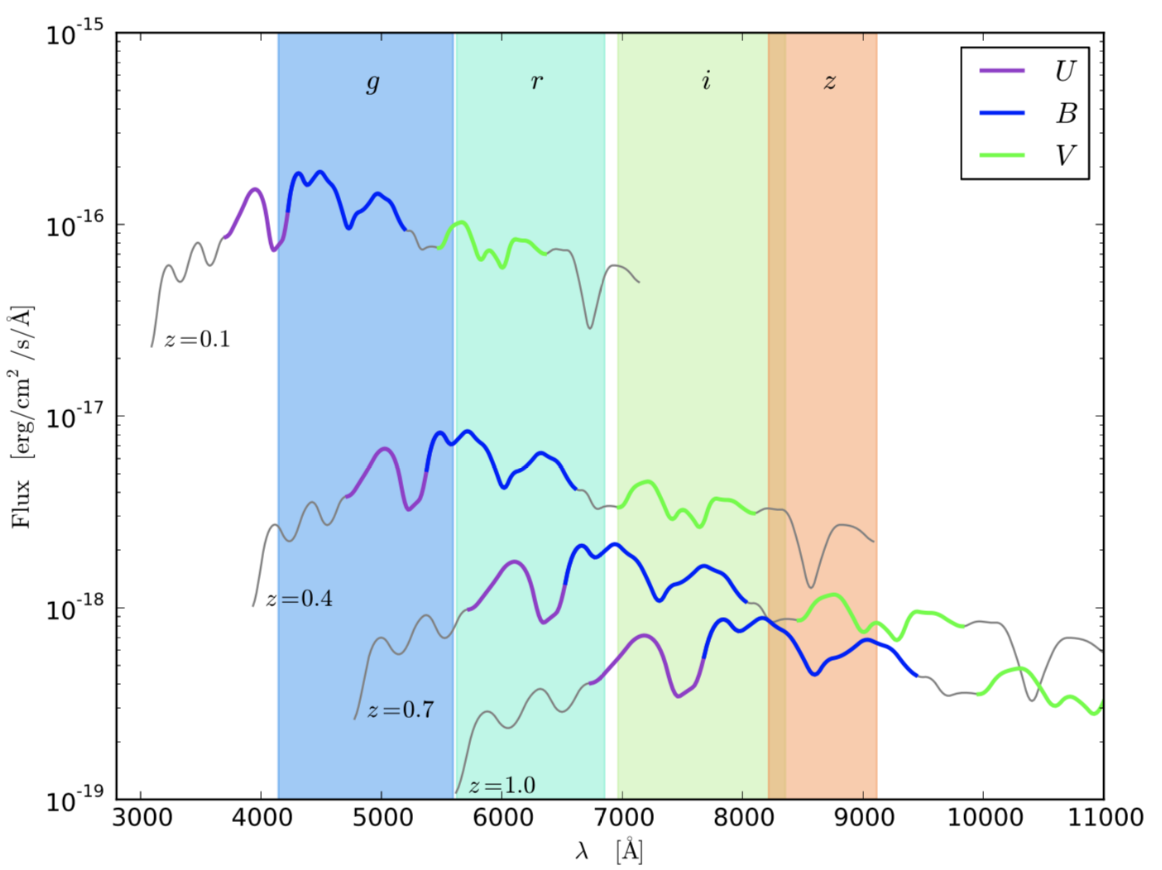
\includegraphics[width=1\textwidth]{MainLayout/NaCl_chapter/figures/flux_evolution.png}
    \caption{Examples of four spectra at different redshifts 0.1, 0.4, 0.7 and 1.0. The highlighted parts of the spectra represent restframe band would measure. The highlighted areas on the graph are the regions where the observer bands measure.}
    \label{fig:flux_evolution}
\end{figure}

The classic approach to convert the observed fluxes and magnitudes into restframe is to apply a K-correction \cite{hogg2002kcorrection}. This allows us to compare observed
fluxes in the same restframe band which is essential to modeling type Ia supernova and measuring the cosmic expansion. The idea is to then describe the supernova magnitude
in the restframe $B^*$ where Type Ia supernovae are standardizable. \\

We define the restframe spectral flux density surface $\mathcal{S}(\lambda, p)$ the spectrophotometric evolution of Type Ia supernova. This will be the quantity that we will
be determining in order to measure the supernovae distances. It's important to note that the spectral flux density $\mathcal{S}$ is determined empirically as the efforts to develop a realistic theoretical 
description of the spectral flux density are extremely difficult (\cite{Blinnikov_2006_difficult_theory}, \cite{R_pke_2018_difficult_theory},  
\cite{Pakmor_2024_difficult_theory}). It's also important to note that we need to use both spectral and photometric data. 
The reason for that is that it is difficult to obtain spectral data over a large phase range and it is to difficult to accurately calibrate the spectra. 
The photometric data then becomes crucial to infer distances while spectra allow us to determine the fine features of the model.\\


\subsection{Models trained on photometric \& spectroscopic datasets}

Here we present some of the empirical spectrophotometric models as well the state of the art SALT models.\\

\noindent \textbf{\underline{MLCS2k2}} \\

The MLCS2k2 model (\textit{Multicolor Light-Curve Shapes 2002}) was 
developed for the analysis of the \textit{High-Z Supernova Search Team} (\cite{Riess_1996}). It describes the observed magnitude of a supernova at a 
specific time phase. The model directly fits a series of functions that describes the lightcurves in a specific band as well as multiple parameters 
including the time of maximum emission of light in the B band restframe $ t_{max}^B$ and an error model. This is the only model I will be
describing here that gets adjusted to describe a function that describes the data. The other models are directly fitted
on the data. It is important to note that there isn't a parameter that describes the supernova color variation since it is assumed 
to be associated with the galactic dust extinction. Before adjusting the 
model parameters, a K-correction is applied to every supernova. \\

\noindent \textbf{\underline{SALT/SALT2/SALT3}} \\

The SALT model (Spectral Adaptative Light curve Template, \cite{Guy_2005}) was developed for the analysis of the SNLS data. The spectral surface $\mathcal{S}(\lambda, p)$
was designed to be capable of varying with 2 parameters that represent the stretch and color of the supernova. This was the first model to include a global parameterization of
supernovae.
The SALT model was pushed further with SALT2 (\cite{Guy_2007_SALT2}) by applyig a Principal Component Analysis (PCA) . This was done by modeling $\mathcal{S}(\lambda, p)$ with two 2-D
surfaces that are described by a base of splines. It's important to note that in SALT2 no K-corrections are applied, instead an offset in the $B^*$ is applied and the measured 
fluxes are brought to restframe. Finally, a later model was publish with the exact same parameterization of SALT2 called SALT3 (\cite{Kenworthy_2021_SALT3}) where the model was
retrained on a larger dataset. \\

\subsection{Models trained on the SNfactory dataset}

SNfactory is a survey that ran from 2004 to 2014 collecting a sequences of spectra of nearby supernovae over a long period of time, thus making the SNfactory dataset (\cite{snfactory}). This is the only dataset that contains a fine spectroscopic description in a large phase range. The well calibrated spectra in the SNfactory dataset will also mean that it doesn't need to be accompanied by photometric measurements to measure distances. \\
These features makes this dataset unique and very interesting to use in order to study the properties of supernova. However it cannot be used alone to measure cosmological parameters such as $w$ since the furthest supernova is at redshift $z\approx0.11$. \


\noindent \textbf{\underline{SNEMO}} \\

SNEMO model (SuperNova Empirical MOdels, \cite{Saunders_2018_SNEMO}) generalises the PCA used in SALT2. In SNEMO, the $\mathcal{S}(\lambda, p)$ components are extracted
using an Expectation Minimization for Factor Analysis or EMFA that takes into account the measurement uncertainties that affects the model. With SNEMO 
multiple model trainings can be done at different orders. At the second order, the $\mathcal{S}(\lambda, p)$ is described with 2 parameters that represent the color and
stretch of the supernova where comparisons with the SALT2 color and stretch parameters have shown strong correlations. \\ 

\noindent \textbf{\underline{SUGAR}} \\

SUGAR (SUpernova Generator And Reconstructor, \cite{L_get_2020_SUGAR}) uses EMFA like SNEMO but applied in a different space with the idea that
supernova variability is encoded in their spectral data. The founders of SUGAR have chosen 13 spectral feautres to identify the supernova variability. The work
with SUGAR has essentially showed that the supernova variability can be captured by 3 parameters, one more than the traditional stretch and color parameters. \\

\noindent \textbf{\underline{Twins Embedding}} \\

The Twins Embedding model (\cite{Boone_2021_twins_embedding}) uses a non-linear parameterization to describe the supernova diversity. It uses a new standardization
method based on the spectral differences between supernova at specific regions. This is also called the spectral distance. If the spectral distance between two supernovae is
small enough they are considered as "Twins". The model is adjusted using an algorithm that does non-linear dimensionality reduction called Isomap which is a generalization of 
PCA while accounting for non-linearities. \\

\noindent \textbf{\underline{SuPAErnova}} \\

The SuPAErnova model (\cite{Stein_2022_PAE}) uses a probabilistic autoencoder in order to assess the supernova diversity. The use of machine learning (ML) in this case 
leaves the model free to explore different ways to determine the necessary parameterization in order to describe the data. The only setback is that it then becomes difficult
to have a physical interpretation of the final parameters. \\